\documentclass[12pt]{article}
\usepackage{graphicx}
\usepackage[a4paper, margin=1in]{geometry}
\usepackage{amsmath}
\usepackage[utf8]{inputenc}
\usepackage{listings}
\usepackage{xcolor}

\usepackage{amsfonts}
\usepackage{amssymb}
\usepackage{geometry}
\usepackage{titlesec}
\usepackage{fancyhdr}
\usepackage{lipsum}


\lstdefinestyle{mystyle}{
    backgroundcolor=\color{white},
    commentstyle=\color{codegreen},
    keywordstyle=\color{magenta},
    numberstyle=\tiny\color{codegray},
    stringstyle=\color{codepurple},
    basicstyle=\ttfamily\footnotesize,
    breakatwhitespace=false,
    breaklines=true,
    captionpos=b,
    keepspaces=true,
    numbers=left,
    numbersep=5pt,
    showspaces=false,
    showstringspaces=false,
    showtabs=false,
    tabsize=2
}

\lstset{style=mystyle}

\definecolor{codegreen}{rgb}{0,0.6,0}
\definecolor{codegray}{rgb}{0.5,0.5,0.5}
\definecolor{codepurple}{rgb}{0.58,0,0.82}

% Configuración de página
\geometry{a4paper, margin=1in}
\pagestyle{fancy}
\fancyhf{}
\rhead{Eidan Owen Plata Salinas}
\lhead{Regresión Logística en Dataset Multiclase}
\cfoot{\thepage}

% Títulos
\titleformat{\section}[block]{\normalfont\Large\bfseries}{\thesection}{1em}{}
\titlespacing*{\section}{0pt}{\baselineskip}{\baselineskip}

% Metadatos
\title{Regresión Logística en Dataset Multiclase}
\author{Eidan Owen Plata Salinas}
\date{\today}


\title{Regresión Logística en Dataset multiclase}
\author{Plata Salinas Eidan Owen}
\date{\today}

\begin{document}
\maketitle
\pagebreak

\section*{Introducción}
El machine learning, o aprendizaje automático, es una rama de la inteligencia artificial que se centra en la construcción de sistemas que pueden aprender de datos. Dentro de este campo.

La regresión logística es un método estadístico utilizado para modelar y analizar conjuntos de datos en los que la variable de respuesta es categórica. Es especialmente útil cuando la variable de respuesta es binaria. 

En este reporte, se explora una implementación de regresión logística en cascada para abordar un problema de clasificación de tres categorías. Para el data set se descargó uno de la pagina  https://archive.ics.uci.edu/dataset/212/vertebral+column sobre columnas vertebrales, que se clasifican en 3 categorias, DH (Disk Hernia), Spondylolisthesis (SL), Normal (NO).

\section*{Desarrollo}
A continuación, se describe el código Python que implementa la regresión logística en cascada. De modo que va comparando si pertenece a 1 clase o al resto, si pertenece al restto entonces agarra esa y la compara con las demas, en este caso al ser 3 clases solo requiere de 2 modelos.
\vspace{1cm}


\subsection*{Clase \texttt{RegresionLogisticaCascada}}
Esta clase emplea dos clasificadores de regresión logística en una estructura de cascada.
\vspace{1cm}

\begin{lstlisting}[language=Python]
class RegresionLogisticaCascada:
    def __init__(self):
        self.clasificador_dh = RegresionLogistica(tasa_aprendizaje=0.01, num_iteraciones=1000)
        self.clasificador_sl = RegresionLogistica(tasa_aprendizaje=0.01, num_iteraciones=1000)

    def entrenar(self, X, y):
        y_dh = np.where(y == 'DH', 1, 0)
        self.clasificador_dh.entrenar(X, y_dh)
        mascara = y != 'DH'
        X_sl = X[mascara]
        y_sl = np.where(y[mascara] == 'SL', 1, 0)
        self.clasificador_sl.entrenar(X_sl, y_sl)

    def predecir(self, X):
        predicciones = []

        predicciones_dh = self.clasificador_dh.predecir(X)
        predicciones_sl = self.clasificador_sl.predecir(X)

        for idx, (prediccion_dh, prediccion_sl) in enumerate(zip(predicciones_dh, predicciones_sl)):
            if prediccion_dh == 1:
                etiqueta = 'DH'
            elif prediccion_sl == 1:
                etiqueta = 'SL'
            else:
                etiqueta = 'NO'
            predicciones.append(etiqueta)
            print(f"Dato {idx+1}: {X.iloc[idx].values} -> Etiqueta predicha: {etiqueta}")

        return np.array(predicciones)

    def obtener_pesos(self):
        return {
            "pesos_clasificador_dh": self.clasificador_dh.pesos,
            "sesgo_clasificador_dh": self.clasificador_dh.sesgo,
            "pesos_clasificador_sl": self.clasificador_sl.pesos,
            "sesgo_clasificador_sl": self.clasificador_sl.sesgo
        }
        
    def graficar_modelo(self, X, y):
        pca = PCA(n_components=3)
        X_pca = pca.fit_transform(X)

        fig = plt.figure(figsize=(10, 8))
        ax = fig.add_subplot(111, projection='3d')
        for etiqueta, color in [('DH', 'red'), ('SL', 'blue'), ('NO', 'green')]:
            mascara = y == etiqueta
            ax.scatter(X_pca[mascara][:, 0], X_pca[mascara][:, 1], X_pca[mascara][:, 2], c=color, label=etiqueta, depthshade=True)

        ax.set_xlabel('Principal Component 1')
        ax.set_ylabel('Principal Component 2')
        ax.set_zlabel('Principal Component 3')
        ax.legend()
        ax.set_title('Modelo de Regresion Logistica en Cascada (3D PCA)')
        plt.show()
\end{lstlisting}
\vspace{1cm}

Aquí, se inician dos clasificadores, uno para 'DH' y otro para 'SL'. Durante el entrenamiento, primero se entrena el clasificador 'DH' y luego el 'SL', usando solo los datos no clasificados como 'DH', para distingirlos entre 'SL' o 'NO'.

Tiene su constructor donde crea 2 instancias de la clase de regresion logistica que veremos más adelante.

El metodo entrenar recibe el dataset y lo evalúa en las 2 instancias antes creadas para obtener los modelos.

El metodo predecir recibe los datos de prueba 'X' y devuelve sus etiquetas.

El metodo obtener pesos simplemente imprime lospesos de los 2 modelos.

El metodo graficar genera una representacion enn tres dimensiones de los modelos uttilizando la librería PCA, que reduce la dimensionalidad del datasett de 5 a 3 variables. 

\vspace{1cm}

\subsection*{Clase \texttt{RegresionLogistica}}
Esta clase es una implementación de la regresión logística binaria.
\vspace{1cm}

\begin{lstlisting}[language=Python]
class RegresionLogistica:
    def __init__(self, tasa_aprendizaje=0.001, num_iteraciones=1000):
        self.tasa_aprendizaje = tasa_aprendizaje
        self.num_iteraciones = num_iteraciones
        self.pesos = None
        self.sesgo = None

    def _sigmoid(self, z):
        return 1 / (1 + np.exp(-z))

    def entrenar(self, X, y):
        num_muestras, num_caracteristicas = X.shape
        self.pesos = np.zeros(num_caracteristicas)
        self.sesgo = 0
        for _ in range(self.num_iteraciones):
            modelo = np.dot(X, self.pesos) + self.sesgo
            predicciones = self._sigmoid(modelo)
            dw = (1 / num_muestras) * np.dot(X.T, (predicciones - y))
            db = (1 / num_muestras) * np.sum(predicciones - y)
            self.pesos -= self.tasa_aprendizaje * dw
            self.sesgo -= self.tasa_aprendizaje * db

    def predecir(self, X):
        modelo = np.dot(X, self.pesos) + self.sesgo
        predicciones = self._sigmoid(modelo)
        y_pred = [1 if i > 0.5 else 0 for i in predicciones]
        return np.array(y_pred)
\end{lstlisting}
\vspace{1cm}

En esta clase, se implementan las funciones básicas para entrenar y predecir utilizando la regresión logística con el sigmoide como metodo para pasar a binario los datos del dataset.

\vspace{1cm}

\subsection*{Función \texttt{dat\_a\_csv}}
Esta función convierte un archivo \texttt{.dat} en un archivo \texttt{.csv}.
\vspace{1cm}

\begin{lstlisting}[language=Python]
def dat_a_csv(nombre_archivo_dat, nombre_archivo_csv):
    with open(nombre_archivo_dat, 'r') as archivo_dat:
        lineas = archivo_dat.readlines()
        with open(nombre_archivo_csv, 'w', newline='') as archivo_csv:
            escritor = csv.writer(archivo_csv, delimiter=',')
            for linea in lineas:
                datos = linea.split()[:]
                escritor.writerow(datos)
\end{lstlisting}
\vspace{1cm}

La función lee el archivo \texttt{.dat} obtenido de la pagina de datasets, extrae los datos y los escribe en un nuevo archivo \texttt{.csv}

\vspace{1cm}

\subsection*{Función \texttt{csv\_a\_datos}}
Esta función convierte un archivo \texttt{.csv} en una cadena de texto.
\vspace{1cm}

\begin{lstlisting}[language=Python]
def csv_a_datos(nombre_archivo):
    datos = []
    with open(nombre_archivo, newline='') as archivo_csv:
        lector_csv = csv.reader(archivo_csv, delimiter=',')
        for fila in lector_csv:
            datos.append(','.join(fila))

    datos_csv = '\n'.join(datos)
    return datos_csv
\end{lstlisting}
\vspace{1cm}

La función lee el archivo \texttt{.csv} y devuelve su contenido en formato de cadena para ser leido por la funcion precesar.

\vspace{1cm}

\subsection*{Función \texttt{procesar\_csv}}
Esta función procesa la cadena de texto antes extraida para obtener conjuntos de entrenamiento y prueba.
\vspace{1cm}

\begin{lstlisting}[language=Python]
def procesar_csv(datos: str):
    from io import StringIO
    datos_io = StringIO(datos)
    df = pd.read_csv(datos_io, header=None)
    X = df.iloc[:, :-1]
    y = df.iloc[:, -1]
    X_entrenamiento, X_prueba, y_entrenamiento, y_prueba = train_test_split(X, y, test_size=0.2, random_state=42)

    return X_entrenamiento, X_prueba, y_entrenamiento, y_prueba

\end{lstlisting}
\vspace{1cm}

Convierte la cadena de texto en un dataframe de pandas y divide los datos en los segmentos requeridos para poner a prueba el programa, que consisten en los vectores característicos, las etiquetas y datos para probar el modelo más adelante.

\vspace{1cm}

\subsection*{Código principal}

\begin{lstlisting}[language=Python]
nombre_archivo_dat = 'datata.dat'
nombre_archivo_csv = 'conjunto.csv'
dat_a_csv(nombre_archivo_dat, nombre_archivo_csv)
X_entrenamiento, X_prueba, y_entrenamiento, y_prueba = procesar_csv(csv_a_datos('conjunto.csv'))
clasificador_cascada = RegresionLogisticaCascada()
clasificador_cascada.entrenar(X_entrenamiento, y_entrenamiento)
info_pesos = clasificador_cascada.obtener_pesos()
print(info_pesos)

y_predicha = clasificador_cascada.predecir(X_prueba)
precision = np.mean(y_predicha == y_prueba)
print(f"Precision: {precision * 100:.2f}%")
clasificador_cascada.graficar_modelo(X_entrenamiento, y_entrenamiento)

\end{lstlisting}
\vspace{1cm}

Aqui ponemos a funcionar todas las funciones antes discutidas para entrenar el modelo con el dataset, proberlo y graficar los resultados.

\clearpage
\section*{Conclusión}
El programa presentado es un ejemplo claro de cómo la regresión logística puede ser adaptada para manejar problemas de clasificación multi-clase. A través del uso de una estructura en cascada, se puede abordar de efectiva pero quiza no eficiente la tarea de clasificar datos en tres categorías distintas.

Aunque la regresión logística es un modelo simple, con adaptaciones y técnicas adicionales, demuestra ser una herramienta poderosa en el ámbito del aprendizaje automático, incluso con las limitaciones que se vieron en la practica. 

A continuacion los resultados.
\vspace{1cm}\vspace{1cm}
\begin{figure}[h] % Coloca la imagen aquí (h significa aquí)
    \centering
    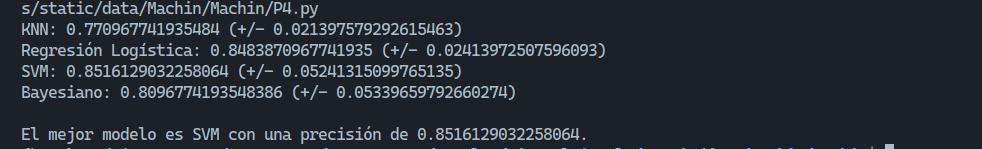
\includegraphics[width=0.6\textwidth]{1.jpg} % Especifica el nombre de la imagen y su ancho relativo al ancho del texto
    \caption{Graficacion de los datos de entrenamiento despues del modelo.} % Agrega una descripción o título a la imagen
    \label{fig:1} % Etiqueta para referenciar la figura en el texto
\end{figure}
\vspace{1cm}\vspace{1cm}
\begin{figure}[h] % Coloca la imagen aquí (h significa aquí)
    \centering
    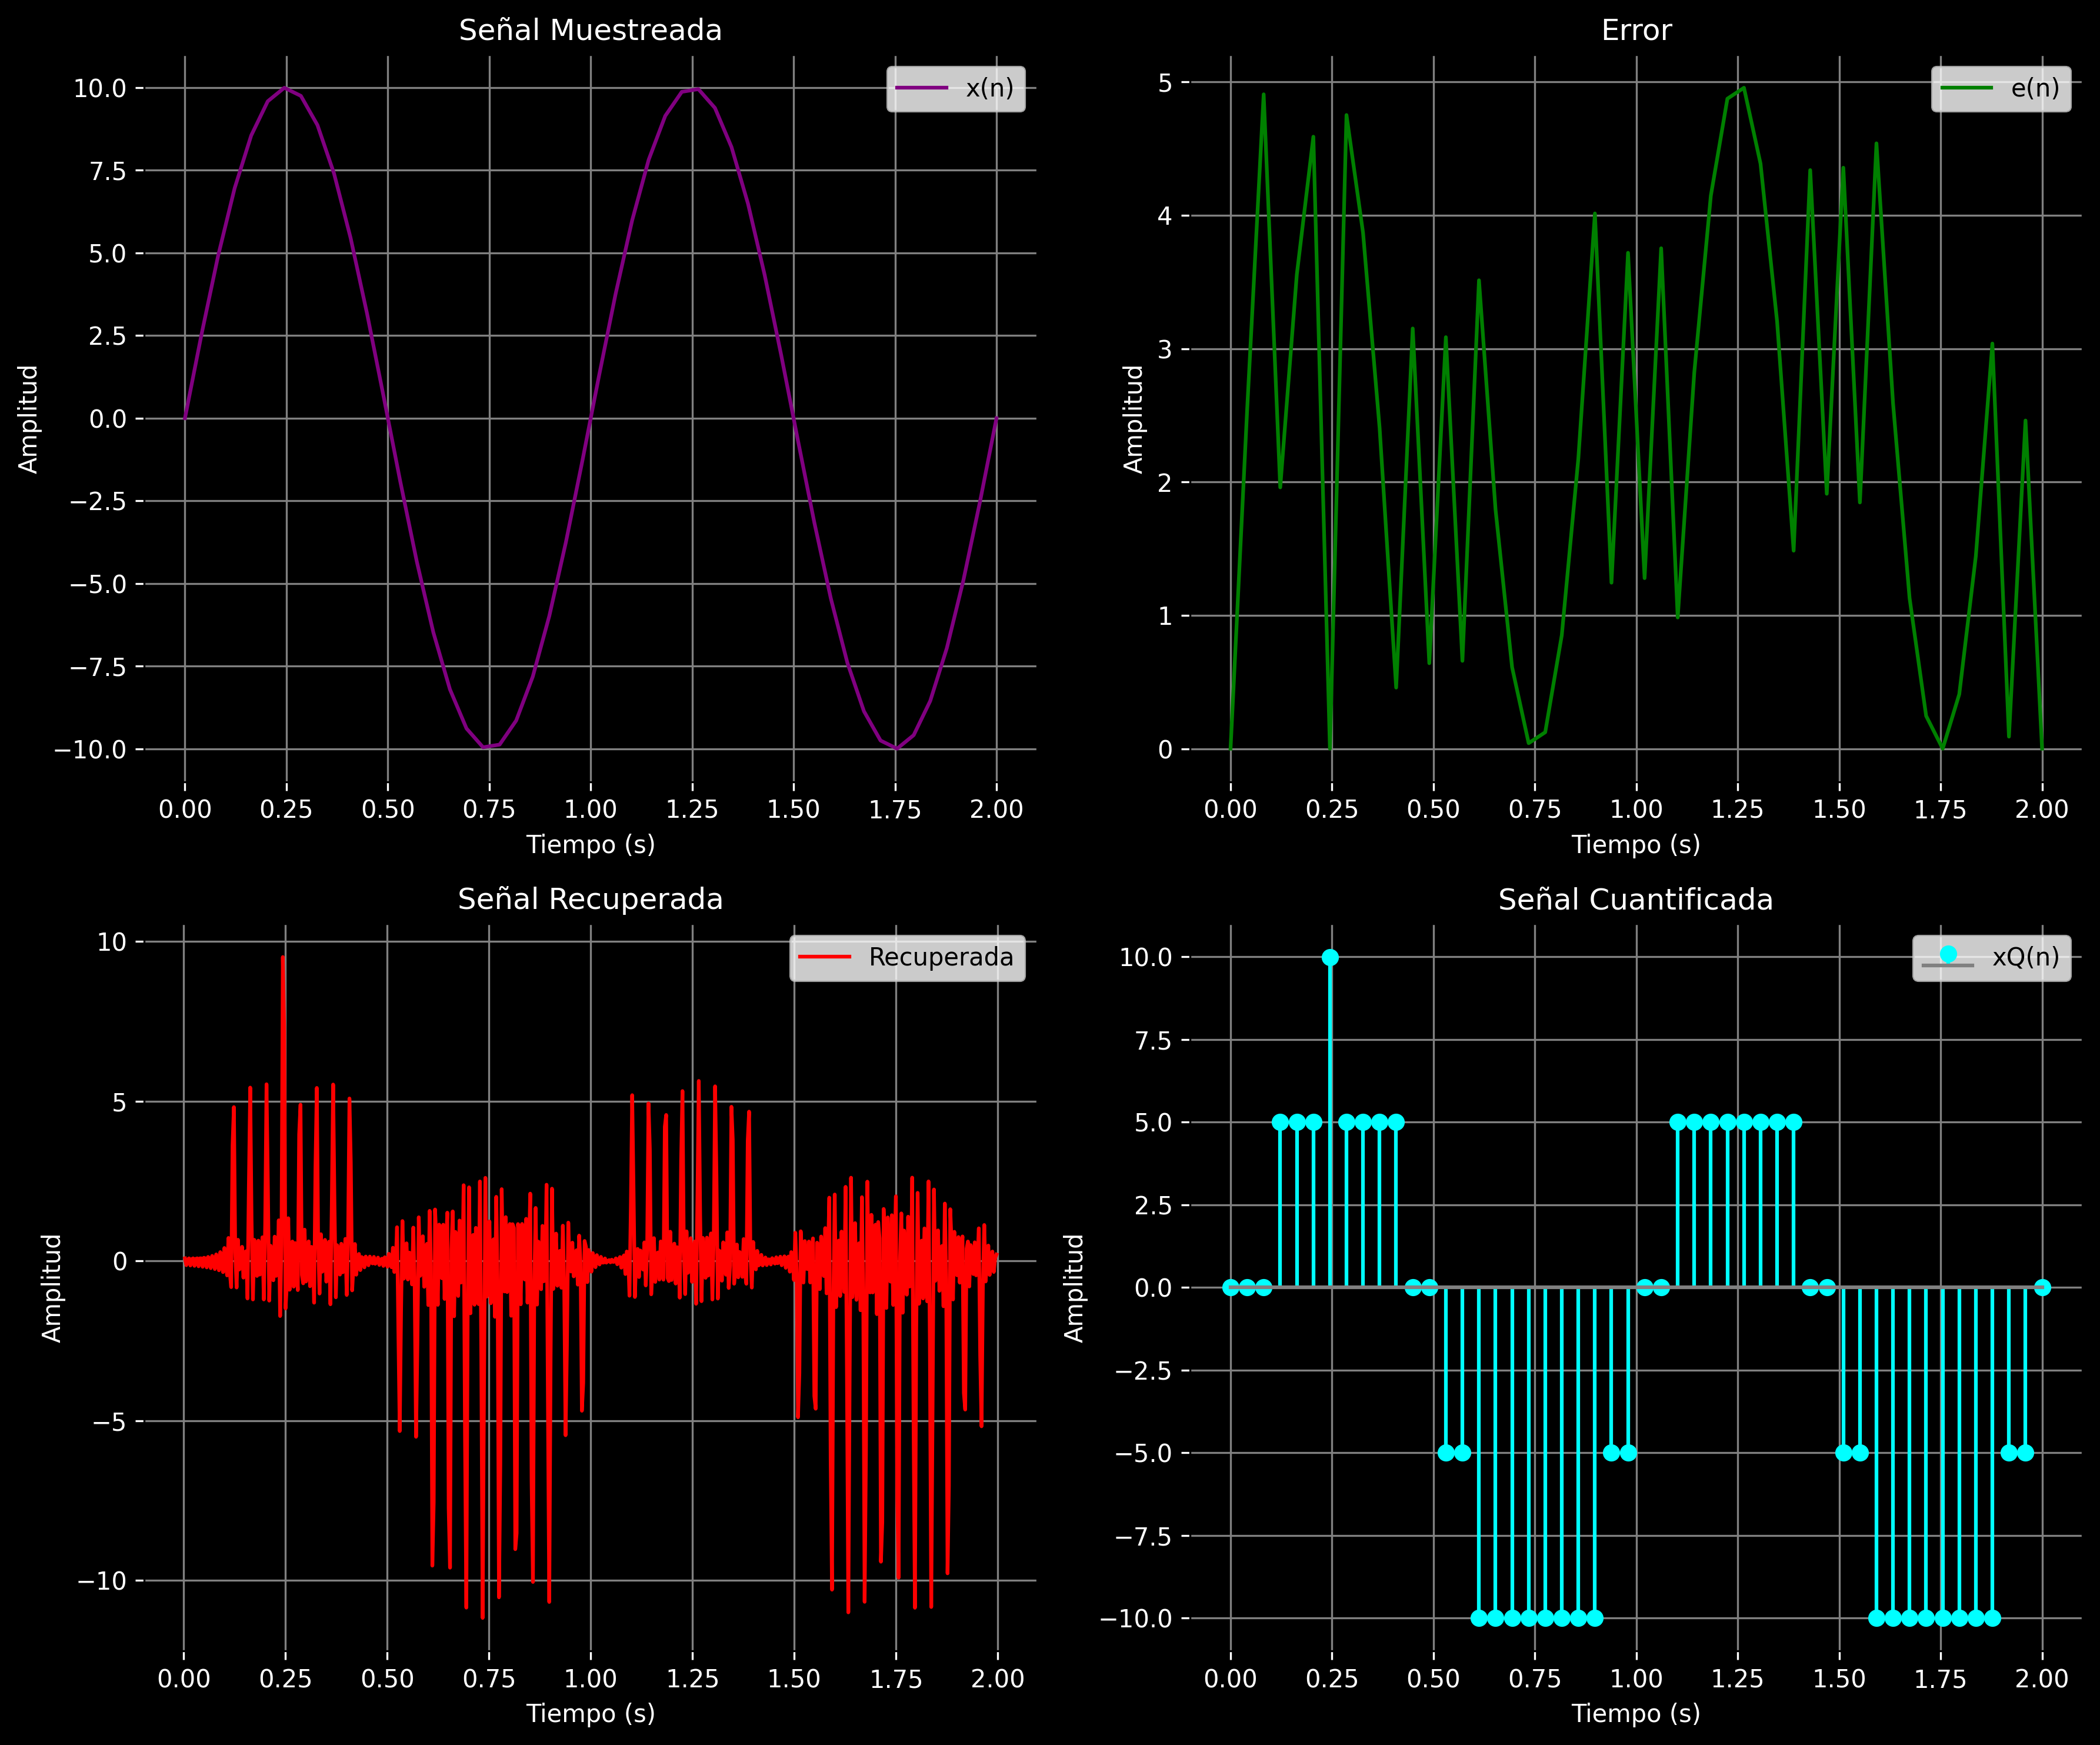
\includegraphics[width=0.99\textwidth]{2.jpg} % Especifica el nombre de la imagen y su ancho relativo al ancho del texto
    \caption{Pesos y evaluacion de datos de prueba.} % Agrega una descripción o título a la imagen
    \label{fig:2} % Etiqueta para referenciar la figura en el texto
\end{figure}


\clearpage
\section*{Codigo completo}
\begin{lstlisting}[language=Python]
import csv
import pandas as pd
from sklearn.model_selection import train_test_split
from sklearn.decomposition import PCA
import numpy as np
import matplotlib.pyplot as plt

class RegresionLogisticaCascada:
    def __init__(self):
        self.clasificador_dh = RegresionLogistica(tasa_aprendizaje=0.01, num_iteraciones=1000)
        self.clasificador_sl = RegresionLogistica(tasa_aprendizaje=0.01, num_iteraciones=1000)

    def entrenar(self, X, y):
        y_dh = np.where(y == 'DH', 1, 0)
        self.clasificador_dh.entrenar(X, y_dh)
        mascara = y != 'DH'
        X_sl = X[mascara]
        y_sl = np.where(y[mascara] == 'SL', 1, 0)
        self.clasificador_sl.entrenar(X_sl, y_sl)

    def predecir(self, X):
        predicciones = []

        predicciones_dh = self.clasificador_dh.predecir(X)
        predicciones_sl = self.clasificador_sl.predecir(X)

        for idx, (prediccion_dh, prediccion_sl) in enumerate(zip(predicciones_dh, predicciones_sl)):
            if prediccion_dh == 1:
                etiqueta = 'DH'
            elif prediccion_sl == 1:
                etiqueta = 'SL'
            else:
                etiqueta = 'NO'
            predicciones.append(etiqueta)
            print(f"Dato {idx+1}: {X.iloc[idx].values} -> Etiqueta predicha: {etiqueta}")

        return np.array(predicciones)

    def obtener_pesos(self):
        return {
            "pesos_clasificador_dh": self.clasificador_dh.pesos,
            "sesgo_clasificador_dh": self.clasificador_dh.sesgo,
            "pesos_clasificador_sl": self.clasificador_sl.pesos,
            "sesgo_clasificador_sl": self.clasificador_sl.sesgo
        }
        
    def graficar_modelo(self, X, y):
        pca = PCA(n_components=3)
        X_pca = pca.fit_transform(X)

        fig = plt.figure(figsize=(10, 8))
        ax = fig.add_subplot(111, projection='3d')
        for etiqueta, color in [('DH', 'red'), ('SL', 'blue'), ('NO', 'green')]:
            mascara = y == etiqueta
            ax.scatter(X_pca[mascara][:, 0], X_pca[mascara][:, 1], X_pca[mascara][:, 2], c=color, label=etiqueta, depthshade=True)

        ax.set_xlabel('Principal Component 1')
        ax.set_ylabel('Principal Component 2')
        ax.set_zlabel('Principal Component 3')
        ax.legend()
        ax.set_title('Modelo de Regresion Logistica en Cascada (3D PCA)')
        plt.show()


class RegresionLogistica:
    def __init__(self, tasa_aprendizaje=0.001, num_iteraciones=1000):
        self.tasa_aprendizaje = tasa_aprendizaje
        self.num_iteraciones = num_iteraciones
        self.pesos = None
        self.sesgo = None

    def _sigmoid(self, z):
        return 1 / (1 + np.exp(-z))

    def entrenar(self, X, y):
        num_muestras, num_caracteristicas = X.shape
        self.pesos = np.zeros(num_caracteristicas)
        self.sesgo = 0
        for _ in range(self.num_iteraciones):
            modelo = np.dot(X, self.pesos) + self.sesgo
            predicciones = self._sigmoid(modelo)
            dw = (1 / num_muestras) * np.dot(X.T, (predicciones - y))
            db = (1 / num_muestras) * np.sum(predicciones - y)
            self.pesos -= self.tasa_aprendizaje * dw
            self.sesgo -= self.tasa_aprendizaje * db

    def predecir(self, X):
        modelo = np.dot(X, self.pesos) + self.sesgo
        predicciones = self._sigmoid(modelo)
        y_pred = [1 if i > 0.5 else 0 for i in predicciones]
        return np.array(y_pred)

def dat_a_csv(nombre_archivo_dat, nombre_archivo_csv):
    with open(nombre_archivo_dat, 'r') as archivo_dat:
        lineas = archivo_dat.readlines()
        with open(nombre_archivo_csv, 'w', newline='') as archivo_csv:
            escritor = csv.writer(archivo_csv, delimiter=',')
            for linea in lineas:
                datos = linea.split()[:]
                escritor.writerow(datos)

def csv_a_datos(nombre_archivo):
    datos = []
    with open(nombre_archivo, newline='') as archivo_csv:
        lector_csv = csv.reader(archivo_csv, delimiter=',')
        for fila in lector_csv:
            datos.append(','.join(fila))

    datos_csv = '\n'.join(datos)
    return datos_csv

def procesar_csv(datos: str):
    from io import StringIO
    datos_io = StringIO(datos)
    df = pd.read_csv(datos_io, header=None)
    X = df.iloc[:, :-1]
    y = df.iloc[:, -1]
    X_entrenamiento, X_prueba, y_entrenamiento, y_prueba = train_test_split(X, y, test_size=0.2, random_state=42)

    return X_entrenamiento, X_prueba, y_entrenamiento, y_prueba

nombre_archivo_dat = 'datata.dat'
nombre_archivo_csv = 'conjunto.csv'
dat_a_csv(nombre_archivo_dat, nombre_archivo_csv)
X_entrenamiento, X_prueba, y_entrenamiento, y_prueba = procesar_csv(csv_a_datos('conjunto.csv'))
clasificador_cascada = RegresionLogisticaCascada()
clasificador_cascada.entrenar(X_entrenamiento, y_entrenamiento)
info_pesos = clasificador_cascada.obtener_pesos()
print(info_pesos)

y_predicha = clasificador_cascada.predecir(X_prueba)
precision = np.mean(y_predicha == y_prueba)
print(f"Precision: {precision * 100:.2f}%")
clasificador_cascada.graficar_modelo(X_entrenamiento, y_entrenamiento)

\end{lstlisting}

\end{document}
